% Options for packages loaded elsewhere
\PassOptionsToPackage{unicode}{hyperref}
\PassOptionsToPackage{hyphens}{url}
%
\documentclass[
]{article}
\usepackage{amsmath,amssymb}
\usepackage{lmodern}
\usepackage{ifxetex,ifluatex}
\ifnum 0\ifxetex 1\fi\ifluatex 1\fi=0 % if pdftex
  \usepackage[T1]{fontenc}
  \usepackage[utf8]{inputenc}
  \usepackage{textcomp} % provide euro and other symbols
\else % if luatex or xetex
  \usepackage{unicode-math}
  \defaultfontfeatures{Scale=MatchLowercase}
  \defaultfontfeatures[\rmfamily]{Ligatures=TeX,Scale=1}
\fi
% Use upquote if available, for straight quotes in verbatim environments
\IfFileExists{upquote.sty}{\usepackage{upquote}}{}
\IfFileExists{microtype.sty}{% use microtype if available
  \usepackage[]{microtype}
  \UseMicrotypeSet[protrusion]{basicmath} % disable protrusion for tt fonts
}{}
\makeatletter
\@ifundefined{KOMAClassName}{% if non-KOMA class
  \IfFileExists{parskip.sty}{%
    \usepackage{parskip}
  }{% else
    \setlength{\parindent}{0pt}
    \setlength{\parskip}{6pt plus 2pt minus 1pt}}
}{% if KOMA class
  \KOMAoptions{parskip=half}}
\makeatother
\usepackage{xcolor}
\IfFileExists{xurl.sty}{\usepackage{xurl}}{} % add URL line breaks if available
\IfFileExists{bookmark.sty}{\usepackage{bookmark}}{\usepackage{hyperref}}
\hypersetup{
  pdftitle={Analysis of the Difference in Means of Systolic Blood Pressure between Smokers and Non-Smokers Using t-Test.},
  pdfauthor={Brock Akerman and Hanan Ali},
  hidelinks,
  pdfcreator={LaTeX via pandoc}}
\urlstyle{same} % disable monospaced font for URLs
\usepackage[margin=1in]{geometry}
\usepackage{color}
\usepackage{fancyvrb}
\newcommand{\VerbBar}{|}
\newcommand{\VERB}{\Verb[commandchars=\\\{\}]}
\DefineVerbatimEnvironment{Highlighting}{Verbatim}{commandchars=\\\{\}}
% Add ',fontsize=\small' for more characters per line
\usepackage{framed}
\definecolor{shadecolor}{RGB}{248,248,248}
\newenvironment{Shaded}{\begin{snugshade}}{\end{snugshade}}
\newcommand{\AlertTok}[1]{\textcolor[rgb]{0.94,0.16,0.16}{#1}}
\newcommand{\AnnotationTok}[1]{\textcolor[rgb]{0.56,0.35,0.01}{\textbf{\textit{#1}}}}
\newcommand{\AttributeTok}[1]{\textcolor[rgb]{0.77,0.63,0.00}{#1}}
\newcommand{\BaseNTok}[1]{\textcolor[rgb]{0.00,0.00,0.81}{#1}}
\newcommand{\BuiltInTok}[1]{#1}
\newcommand{\CharTok}[1]{\textcolor[rgb]{0.31,0.60,0.02}{#1}}
\newcommand{\CommentTok}[1]{\textcolor[rgb]{0.56,0.35,0.01}{\textit{#1}}}
\newcommand{\CommentVarTok}[1]{\textcolor[rgb]{0.56,0.35,0.01}{\textbf{\textit{#1}}}}
\newcommand{\ConstantTok}[1]{\textcolor[rgb]{0.00,0.00,0.00}{#1}}
\newcommand{\ControlFlowTok}[1]{\textcolor[rgb]{0.13,0.29,0.53}{\textbf{#1}}}
\newcommand{\DataTypeTok}[1]{\textcolor[rgb]{0.13,0.29,0.53}{#1}}
\newcommand{\DecValTok}[1]{\textcolor[rgb]{0.00,0.00,0.81}{#1}}
\newcommand{\DocumentationTok}[1]{\textcolor[rgb]{0.56,0.35,0.01}{\textbf{\textit{#1}}}}
\newcommand{\ErrorTok}[1]{\textcolor[rgb]{0.64,0.00,0.00}{\textbf{#1}}}
\newcommand{\ExtensionTok}[1]{#1}
\newcommand{\FloatTok}[1]{\textcolor[rgb]{0.00,0.00,0.81}{#1}}
\newcommand{\FunctionTok}[1]{\textcolor[rgb]{0.00,0.00,0.00}{#1}}
\newcommand{\ImportTok}[1]{#1}
\newcommand{\InformationTok}[1]{\textcolor[rgb]{0.56,0.35,0.01}{\textbf{\textit{#1}}}}
\newcommand{\KeywordTok}[1]{\textcolor[rgb]{0.13,0.29,0.53}{\textbf{#1}}}
\newcommand{\NormalTok}[1]{#1}
\newcommand{\OperatorTok}[1]{\textcolor[rgb]{0.81,0.36,0.00}{\textbf{#1}}}
\newcommand{\OtherTok}[1]{\textcolor[rgb]{0.56,0.35,0.01}{#1}}
\newcommand{\PreprocessorTok}[1]{\textcolor[rgb]{0.56,0.35,0.01}{\textit{#1}}}
\newcommand{\RegionMarkerTok}[1]{#1}
\newcommand{\SpecialCharTok}[1]{\textcolor[rgb]{0.00,0.00,0.00}{#1}}
\newcommand{\SpecialStringTok}[1]{\textcolor[rgb]{0.31,0.60,0.02}{#1}}
\newcommand{\StringTok}[1]{\textcolor[rgb]{0.31,0.60,0.02}{#1}}
\newcommand{\VariableTok}[1]{\textcolor[rgb]{0.00,0.00,0.00}{#1}}
\newcommand{\VerbatimStringTok}[1]{\textcolor[rgb]{0.31,0.60,0.02}{#1}}
\newcommand{\WarningTok}[1]{\textcolor[rgb]{0.56,0.35,0.01}{\textbf{\textit{#1}}}}
\usepackage{longtable,booktabs,array}
\usepackage{calc} % for calculating minipage widths
% Correct order of tables after \paragraph or \subparagraph
\usepackage{etoolbox}
\makeatletter
\patchcmd\longtable{\par}{\if@noskipsec\mbox{}\fi\par}{}{}
\makeatother
% Allow footnotes in longtable head/foot
\IfFileExists{footnotehyper.sty}{\usepackage{footnotehyper}}{\usepackage{footnote}}
\makesavenoteenv{longtable}
\usepackage{graphicx}
\makeatletter
\def\maxwidth{\ifdim\Gin@nat@width>\linewidth\linewidth\else\Gin@nat@width\fi}
\def\maxheight{\ifdim\Gin@nat@height>\textheight\textheight\else\Gin@nat@height\fi}
\makeatother
% Scale images if necessary, so that they will not overflow the page
% margins by default, and it is still possible to overwrite the defaults
% using explicit options in \includegraphics[width, height, ...]{}
\setkeys{Gin}{width=\maxwidth,height=\maxheight,keepaspectratio}
% Set default figure placement to htbp
\makeatletter
\def\fps@figure{htbp}
\makeatother
\setlength{\emergencystretch}{3em} % prevent overfull lines
\providecommand{\tightlist}{%
  \setlength{\itemsep}{0pt}\setlength{\parskip}{0pt}}
\setcounter{secnumdepth}{-\maxdimen} % remove section numbering
\ifluatex
  \usepackage{selnolig}  % disable illegal ligatures
\fi

\title{Analysis of the Difference in Means of Systolic Blood Pressure
between Smokers and Non-Smokers Using t-Test.}
\author{Brock Akerman and Hanan Ali}
\date{ST502 - Spring 2022}

\begin{document}
\maketitle

A sample of data is extracted from the Framingham Heart Study which
includes the systolic blood pressure of participants who are identified
as either smokers or non-smokers. Smokers in this study are defined as
participants who have smoked cigarettes anytime the year preceding the
physical examination while non-smokers are those who have abstained from
smoking during that same period of time (Magnani, 2017). The data
contains a column of qualitative binary values characterizing the
subjects smoking habit and a second column pairing it with a single
measurement of systolic blood pressure measured in millimeters of
mercury (mmHg).

We are interested in making inference about the difference in blood
pressure means between smokers and non-smokers. To test whether a
difference between means exists we will utilize the pooled t-test and
the Welch-Satterthwaite t-test. Random sampling and a normal
distribution are assumed for our samples; however, examining plots of
the data before conducting any t-tests is good practice. If assumptions
about samples are made and there is an opportunity to strengthen the
results of our test by reinforcing those assumptions we should do so.\\
~\\

\begin{center}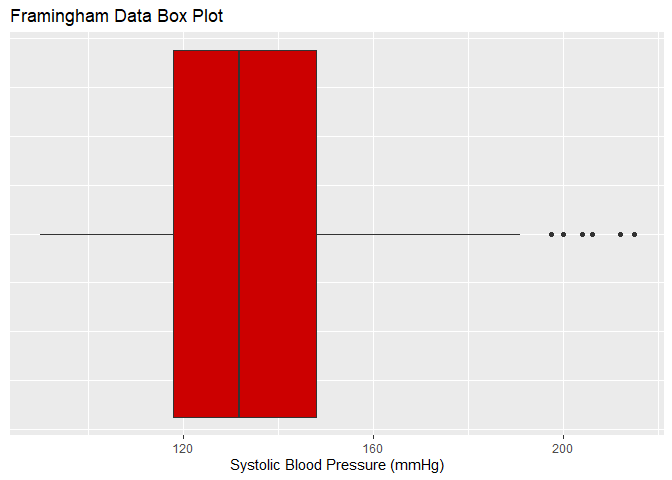
\includegraphics{Project1_files/figure-latex/unnamed-chunk-5-1} \end{center}

\hfill\break
\hfill\break

\begin{center}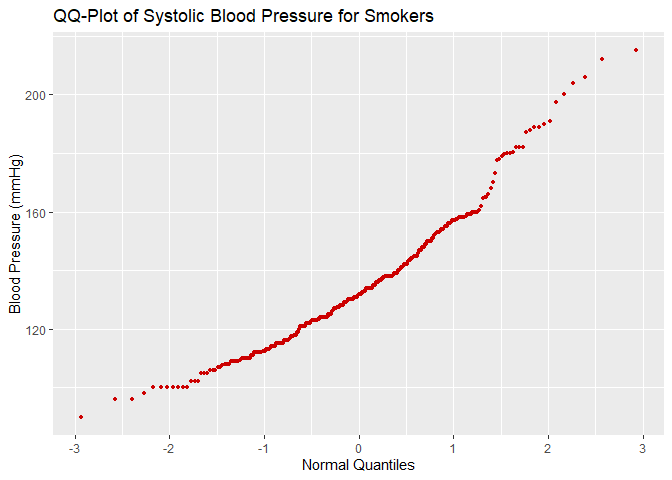
\includegraphics{Project1_files/figure-latex/unnamed-chunk-6-1} \end{center}

\hfill\break
\hfill\break

\begin{center}\includegraphics{Project1_files/figure-latex/unnamed-chunk-7-1} \end{center}

\hfill\break
\hfill\break

Visually summarizing the histogram shows a skew toward the right. There
was the presence of outliers influencing the distribution and causing an
observable skew. The concerning values are systolic blood pressure
observations where the subject had a 180 mmHg reading or higher. A
pressure observed above 180mmHg is consider a medical emergency and
requires urgent care and hospitalization (Heart.org, 2017).\\
~\\
The Quantile-Quantile plot exhibits a linear tendency though variability
in observations in the right tail may be distorting linearity. It is not
enough to reject the normality assumption on this fact alone though
purging outliers would serve to strengthen the argument in favor of
assuming normality.\\
~\\
I produced a boxplot to examine the distribution and highlight outliers.
We found six values that were outside of the interquartile multiplier
range--five observations from the non-smokers sample and one observation
from the smokers sample group. We will report both t-tests with outliers
and without outliers for comparison.\\
~\\

\begin{center}\includegraphics{Project1_files/figure-latex/unnamed-chunk-8-1} \end{center}

\hfill\break
\hfill\break

\begin{center}\includegraphics{Project1_files/figure-latex/unnamed-chunk-9-1} \end{center}

\hfill\break
\hfill\break
After removing the outliers we can see that the histogram looks more
normalized when compared to the histogram with outliers. The skew is
gentler and better representative of the data overall. Likewise, the Q-Q
plot appears slightly more linear than before. The preliminary analysis
is complete and we are ready to use our t-tests to make inference on our
sampled means.\\
~\\

\hypertarget{pooled-t-test-outliers-included}{%
\subsubsection{Pooled T-test (outliers
included)}\label{pooled-t-test-outliers-included}}

\hypertarget{p-value}{%
\subparagraph{\texorpdfstring{\textbf{P-Value}}{P-Value}}\label{p-value}}

\hfill\break
\(H_{0}: \mu_{1}-\mu_{2} = 0\), There is no difference between means of
smokers and non-smokers.\\
\(H_{0}: \mu_{1}-\mu_{2} ≠ 0\), There is a difference between means of
smokers and non-smokers.\\
~\\
~\\
\(\bar{X}_{1} = \frac{1}{225}\sum(x_{1},x_{2},...,x_{225}) = 137.22444\)\\
\(s^2_{1} = \frac{1}{225^2}\sum^{225}_{i=1}(x_{i}-\bar{x_{1}}) = 562.1447\)\\
\(n_{1} = 225\)\\
~\\
~\\
\(\bar{X}_{2} = \frac{1}{75}\sum(x_{1},x_{2},...,x_{75}) = 128.06667\)\\
\(s^2_{2} = \frac{1}{75^2}\sum^{75}_{j=1}(x_{j}-\bar{x_{2}}) = 352.2117\)\\
\(n_{2} = 75\)\\
~\\
~\\
\(S^2_{p} = \frac{(n_{1}-1)S^2_{1}+(n_{2}-1)S^2_{2}}{n_{1}+n_{2}-2} = \frac{(225-1)562.1447+(75-1)352.2117}{225+75-2} = 510.01370\)\\
~\\
\(S_{p} = \sqrt(S^2_{p}) = \sqrt(510.01370) = 22.58350\)\\
~\\
\(T = \frac{\bar{X_{1}} - \bar{X_{2}}} {S_{p}\sqrt(\frac{1}{n_{1}}+\frac{1}{n_{2}})} = \frac{137.22444 - 128.06667} {22.5835\sqrt(\frac{1}{225}+\frac{1}{75})} = 3.0413\)\\
~\\
Under the null hypothesis, \(H_{0}: T \sim t_{298}\). The rejection
region for the test \(H_{a}: \mu_{1}-\mu_{2} ≠ D_{0}:\)\\
~\\
Rejection Region: \({t_{obs} : |t_{obs}| > t_{\frac{\alpha}{2},df}}\)\\
Rejection Region: \({t_{obs} : |3.04131| > 1.96796}\)\\
~\\
P-Value (two-tailed):\\
\(2*(1-pt(T = 3.0413,df = n_{1}+n_{2}-2)) = 2*(1-0.9987) = 0.00258\)\\
~\\

\textbf{Conclusion:}

Reject \(H_{0}\). At the 0.05 significance level, there is sufficient
evidence to support the claim that mean systolic blood pressure between
smokers and non-smokers is different.\\
~\\
~\\

\hypertarget{confidence-interval}{%
\subparagraph{\texorpdfstring{\textbf{Confidence
Interval}}{Confidence Interval}}\label{confidence-interval}}

\hfill\break
Lower\_Bound\\
\((\bar{X_{1}}-\bar{X_{2}}) - t_{(\frac{\alpha}{2},df)}(S_{p})(\sqrt(\frac{1}{n_{1}}+\frac{1}{n_{2}})) = (137.22444 - 128.06667) - (1.96796)(22.58350)(\sqrt(\frac{1}{225}+\frac{1}{75}) = 3.23194\)\\
~\\
Upper\_Bound\\
\((\bar{X_{1}}-\bar{X_{2}}) + t_{(\frac{\alpha}{2},df)}(S_{p})(\sqrt(\frac{1}{n_{1}}+\frac{1}{n_{2}})) = (137.22444 - 128.06667) + (1.96796)(22.58350)(\sqrt(\frac{1}{225}+\frac{1}{75}) = 15.0835\)\\
~\\

\textbf{Conclusion:}

We are 95\% confident that the mean difference in systolic blood
pressure between smokers and non-smokers is between 3.23194 mmHg and
15.0835 mmHg.\\
~\\
~\\

\hypertarget{pooled-t-test-outliers-omitted}{%
\subsubsection{Pooled T-test (outliers
omitted)}\label{pooled-t-test-outliers-omitted}}

\hypertarget{p-value-1}{%
\subparagraph{\texorpdfstring{\textbf{P-Value}}{P-Value}}\label{p-value-1}}

\hfill\break
\hfill\break
\(H_{0}: \mu_{1}-\mu_{2} = 0\), There is no difference between means of
smokers and non-smokers.\\
\(H_{0}: \mu_{1}-\mu_{2} ≠ 0\), There is a difference between means of
smokers and non-smokers.\\
~\\
~\\
\(\bar{X}_{1} = \frac{1}{220}\sum(x_{1},x_{2},...,x_{220}) = 135.6409\)\\
\(s^2_{1} = \frac{1}{220^2}\sum^{220}_{i=1}(x_{i}-\bar{x_{1}}) = 460.7586\)\\
\(n_{1} = 220\)\\
~\\
~\\
\(\bar{X}_{2} = \frac{1}{74}\sum(x_{1},x_{2},...,x_{74}) = 127.0946\)\\
\(s^2_{2} = \frac{1}{74^2}\sum^{74}_{j=1}(x_{j}-\bar{x_{2}}) = 285.1964\)\\
\(n_{2} = 74\)\\
~\\
~\\
\(S^2_{p} = \frac{(n_{1}-1)S^2_{1}+(n_{2}-1)S^2_{2}}{n_{1}+n_{2}-2} = \frac{(22401)460.7586+(74-1)285.1964}{220+74-2} = 416.868\)\\
~\\
\(S_{p} = \sqrt(S^2_{p}) = \sqrt(416.868) = 20.41735\)\\
~\\
\(T = \frac{\bar{X_{1}} - \bar{X_{2}}} {S_{p}\sqrt(\frac{1}{n_{1}}+\frac{1}{n_{2}})} = \frac{135.6409 - 127.0946} {20.41735\sqrt(\frac{1}{220}+\frac{1}{74})} =3.1148\)\\
~\\
Under the null hypothesis, \(H_{0}: T \sim t_{292}\). The rejection
region for the test \(H_{a}: \mu_{1}-\mu_{2} ≠ D_{0}:\)\\
~\\
Rejection Region: \({t_{obs} : |t_{obs}| > t_{\frac{\alpha}{2},df}}\)\\
Rejection Region: \({t_{obs} : |3.1148| > 1.968121}\)\\
~\\

P-Value (two-tailed):\\
\(2*(1-pt(T = 3.1148,df = 220+74-2)) = 2*(1-0.99898) = 0.00204\)\\
~\\

\textbf{Conclusion:}

Reject \(H_{0}\). At the 0.05 significance level, there is sufficient
evidence to support the claim that mean systolic blood pressure between
smokers and non-smokers is different.\\
~\\
~\\

\hypertarget{confidence-interval-1}{%
\subparagraph{\texorpdfstring{\textbf{Confidence
Interval}}{Confidence Interval}}\label{confidence-interval-1}}

\hfill\break
Lower\_Bound\\
\((\bar{X_{1}}-\bar{X_{2}}) - t_{(\frac{\alpha}{2},df)}(S_{p})(\sqrt(\frac{1}{n_{1}}+\frac{1}{n_{2}})) = (135.6409 - 127.0946) - (1.96796)(20.41735)(\sqrt(\frac{1}{220}+\frac{1}{74}) = 3.14669\)\\
~\\
Upper\_Bound\\
\((\bar{X_{1}}-\bar{X_{2}}) + t_{(\frac{\alpha}{2},df)}(S_{p})(\sqrt(\frac{1}{n_{1}}+\frac{1}{n_{2}})) = (135.6409 - 127.0946) + (1.96796)(20.41735)(\sqrt(\frac{1}{220}+\frac{1}{74}) = 13.9459\)\\
~\\

\textbf{Conclusion:}

We are 95\% confident that the mean difference in systolic blood
pressure between smokers and non-smokers is between 3.14669 mmHg and
13.9459 mmHg.\\
~\\
~\\
~\\
~\\

\hypertarget{welch-satterthwaite-t-test-outliers-included}{%
\subsubsection{Welch-Satterthwaite T-test (outliers
included)}\label{welch-satterthwaite-t-test-outliers-included}}

\hypertarget{p-value-2}{%
\subparagraph{\texorpdfstring{\textbf{P-Value}}{P-Value}}\label{p-value-2}}

For the Welch-Satterthwaite t-test we will test using the same
hypothesis as in the t-test pooled; however, with the assumption about
the variance removed, the test statistic formula.\\
~\\
~\\
\(H_{0}: \mu_{1}-\mu_{2} = 0\), There is no difference between means of
smokers and non-smokers.\\
\(H_{0}: \mu_{1}-\mu_{2} ≠ 0\), There is a difference between means of
smokers and non-smokers.\\
~\\
~\\
\(\bar{X}_{1} = \frac{1}{225}\sum(x_{1},x_{2},...,x_{225}) = 137.22444\)\\
\(s^2_{1} = \frac{1}{225^2}\sum^{225}_{i=1}(x_{i}-\bar{x_{1}}) = 562.1447\)\\
\(n_{1} = 225\)\\
~\\
~\\
\(\bar{X}_{2} = \frac{1}{75}\sum(x_{1},x_{2},...,x_{75}) = 128.06667\)\\
\(s^2_{2} = \frac{1}{75^2}\sum^{75}_{j=1}(x_{j}-\bar{x_{2}}) = 352.2117\)\\
\(n_{2} = 75\)\\
~\\
~\\
\(v = \frac{(\frac{s^2_{1}}{n_{1}}+\frac{s^2_{2}}{n_{2}})^2}{\frac{(\frac{s^2_{1}}{n_{1}})}{n_{1}-1}+{\frac{(\frac{s^2_{2}}{n_{2}})}{n_{2}-1}}} = \frac{(\frac{562.1447}{225}+\frac{352.2117}{75})^2}{\frac{(\frac{562.1447}{225})^2}{225-1}+{\frac{(\frac{352.2117}{75})^2}{75-1}}} = 158.8316\)\\
~\\
\(T = \frac{\bar{X}_1-\bar{X}_2-D_{0}}{\sqrt(\frac{s^2_1}{n_{1}}+\frac{s^2_2}{n_{2}})} = \frac{137.22444-128.06667}{\sqrt(\frac{562.1447}{225}+\frac{352.2117}{75})} = 3.4142\)\\
~\\
Under the null hypothesis,
\(H_{0}: T \sim t_{v,\frac{\alpha}{2}} \sim t_{158.8316,0.025}\). The
rejection region for the test \(H_{a}: \mu_{1}-\mu_{2} ≠ D_{0}:\)\\
~\\
~\\
Rejection Region: \({t_{obs} : |t_{obs}| > t_{0.025,158}}\)\\
~\\
Rejection Region: \({t_{obs} : |3.4142| > 1.9751}\)\\
~\\

P-Value (two-tailed):\\
\(2*(1-pt(T = 3.4142,df = 225+75-2)) = 2*(1-0.9996358) = 0.0007284\)\\
~\\

\textbf{Conclusion:}

Reject \(H_{0}\). At the 0.05 significance level, there is sufficient
evidence to support the claim that mean systolic blood pressure between
smokers and non-smokers is different.

\hypertarget{confidence-interval-2}{%
\subparagraph{\texorpdfstring{\textbf{Confidence
Interval}}{Confidence Interval}}\label{confidence-interval-2}}

\hfill\break
Lower\_Bound\\
\((\bar{X_{1}}-\bar{X_{2}}) - t_{(\frac{\alpha}{2},v)}(\sqrt(\frac{S^2_{1}}{n_{1}}+\frac{S^2_{2}}{n_{2}})) = (137.22444 - 128.06667) - (1.975092)(\sqrt(\frac{562.1447}{225}+\frac{352.2117}{75}) = 3.86004\)\\
~\\
Upper\_Bound\\
\((\bar{X_{1}}-\bar{X_{2}}) + t_{(\frac{\alpha}{2},v)}(\sqrt(\frac{S^2_{1}}{n_{1}}+\frac{S^2_{2}}{n_{2}})) = (137.22444 - 128.06667) + (1.975092)(\sqrt(\frac{562.1447}{225}+\frac{352.2117}{75}) = 14.4555\)\\
~\\

\textbf{Conclusion:}

We are 95\% confident that the mean difference in systolic blood
pressure between smokers and non-smokers is between 3.23194 mmHg and
15.0835 mmHg.\\
~\\
~\\

\hypertarget{welch-satterthwaite-t-test-outliers-omitted}{%
\subsubsection{Welch-Satterthwaite T-test (outliers
omitted)}\label{welch-satterthwaite-t-test-outliers-omitted}}

\hypertarget{p-value-3}{%
\subparagraph{\texorpdfstring{\textbf{P-Value}}{P-Value}}\label{p-value-3}}

\hfill\break

\(H_{0}: \mu_{1}-\mu_{2} = 0\), There is no difference between means of
smokers and non-smokers.\\
\(H_{0}: \mu_{1}-\mu_{2} ≠ 0\), There is a difference between means of
smokers and non-smokers.\\
~\\
~\\
\(\bar{X}_{1} = \frac{1}{220}\sum(x_{1},x_{2},...,x_{220}) = 135.6409\)\\
\(s^2_{1} = \frac{1}{220^2}\sum^{220}_{i=1}(x_{i}-\bar{x_{1}}) = 460.7586\)\\
\(n_{1} = 220\)\\
~\\
~\\
\(\bar{X}_{2} = \frac{1}{74}\sum(x_{1},x_{2},...,x_{74}) = 127.0946\)\\
\(s^2_{2} = \frac{1}{74^2}\sum^{74}_{j=1}(x_{j}-\bar{x_{2}}) = 285.1964\)\\
\(n_{2} = 74\)\\
~\\
~\\
\(v = \frac{(\frac{s^2_{1}}{n_{1}}+\frac{s^2_{2}}{n_{2}})^2}{\frac{(\frac{s^2_{1}}{n_{1}})}{n_{1}-1}+{\frac{(\frac{s^2_{2}}{n_{2}})}{n_{2}-1}}} = \frac{(\frac{460.7586}{220}+\frac{285.1964}{74})^2}{\frac{(\frac{460.7586}{220})^2}{220-1}+{\frac{(\frac{285.1964}{74})^2}{74-1}}} = 158.314\)\\
~\\
\(T = \frac{\bar{X}_1-\bar{X}_2-D_{0}}{\sqrt(\frac{s^2_1}{n_{1}}+\frac{s^2_2}{n_{2}})} = \frac{135.6409-127.0946}{\sqrt(\frac{460.7586}{220}+\frac{285.1964}{74})} = 3.50412\)\\
~\\
Under the null hypothesis,
\(H_{0}: T \sim t_{v,\frac{\alpha}{2}} \sim t_{158.8316,0.025}\). The
rejection region for the test \(H_{a}: \mu_{1}-\mu_{2} ≠ D_{0}:\)\\
~\\

Rejection Region: \({t_{obs} : |t_{obs}| > t_{0.025,158}}\)\\

Rejection Region: \({t_{obs} : |3.50412| > 1.9751}\)\\
~\\

P-Value (two-tailed):\\
\(2*(1-pt(T = 3.50412,df = 220+74-2)) = 2*(1-0.999735) = 0.00053\)\\
~\\

\textbf{Conclusion:}

Reject \(H_{0}\). At the 0.05 significance level, there is sufficient
evidence to support the claim that mean systolic blood pressure between
smokers and non-smokers is different.\\
~\\
~\\

\hypertarget{confidence-interval-3}{%
\subparagraph{\texorpdfstring{\textbf{Confidence
Interval}}{Confidence Interval}}\label{confidence-interval-3}}

\hfill\break
Lower\_Bound\\
\((\bar{X_{1}}-\bar{X_{2}}) - t_{(\frac{\alpha}{2},v)}(\sqrt(\frac{S^2_{1}}{n_{1}}+\frac{S^2_{2}}{n_{2}})) = (135.6409 - 127.0946) - (1.975092)(\sqrt(\frac{460.7586}{220}+\frac{285.1964}{74}) = 3.7292\)\\

Upper\_Bound\\
\((\bar{X_{1}}-\bar{X_{2}}) + t_{(\frac{\alpha}{2},v)}(\sqrt(\frac{S^2_{1}}{n_{1}}+\frac{S^2_{2}}{n_{2}})) = (135.6409 - 127.0946) + (1.975092)(\sqrt(\frac{460.7586}{220}+\frac{285.1964}{74}) = 13.3634\)\\
~\\

\textbf{Conclusion:}

We are 95\% confident that the mean difference in systolic blood
pressure between smokers and non-smokers is between 3.23194 mmHg and
15.0835 mmHg.\\
~\\
~\\

\hypertarget{discussion}{%
\subsubsection{Discussion}\label{discussion}}

Are the mean systolic blood pressures different between smokers and
non-smokers? All four t-test concluded with the same result; a rejection
of the null hypothesis. We found evidence in all four tests of evidence
supporting a difference between systolic blood pressure means of
participants who smoke versus those who do not.

An important step at the beginning of the analysis of our data was the
identification of outliers. We were able to tighten-up the distribution
by removing outliers through a boxplot. Once we saw several observations
that extended beyond the whiskers of the plot, we calculated the
interquartile range and calculated the minimum and maximum values of the
whiskers to find and remove those values that extended past the minimum
and maximum. We now have data more representative of the population of
Framingham, Massachusettes. The histogram return less skewed while the
QQ plot returned more linear.

From the summary below we observe that the p-values for the Pooled
t-tests would result in rejecting the null hypothesis but were closer to
the significance alpha of 0.05 than those from the Satterthwaite
t-tests. Those tests with outliers were closer to the significance alpha
of 0.05 than those p-values from the same tests without the outliers.
What we are finding is that if we were to take many samples, on average
we would find samples would reject more frequently in Satterhwait
t-tests and pooled t-tests. We would would also reject more often with
many samples where outliers were omitted than if they were to remain.

\begin{longtable}[]{@{}lr@{}}
\toprule
Test Type & P-Value \\
\midrule
\endhead
t-Test pooled with outliers & 0.00258 \\
t-Test pooled without outliers & 0.00204 \\
t-Test Satterthwaite with outliers & 0.00073 \\
t-Test Satterthwaite without outliers & 0.00053 \\
\bottomrule
\end{longtable}

Confidence levels list below contain the range of the difference between
each of the means. In our t-Test pooled with outliers had the widest
range of 11.85156 mmHg. Our smallest range was the Satterthwaite t-Test
without outliers with a range of 9.6342 mmHg. The pooled t-test without
outliers and the Satterthwaite t-test with outliers had a very similar
range with a difference of approximately 0.11 mmHg.

\begin{longtable}[]{@{}lrr@{}}
\toprule
Test Type & Lower Bound & Upper Bound \\
\midrule
\endhead
t-Test pooled with outliers & 3.23194 & 15.0835 \\
t-Test pooled without outliers & 3.14669 & 13.9459 \\
t-Test Satterthwaite with outliers & 3.86004 & 14.4555 \\
t-Test Satterthwaite without outliers & 3.7292 & 13.3634 \\
\bottomrule
\end{longtable}

Looking at all the data and summary statistics I would use the
Satterthwaite t-Test with outliers removed. When presenting results;
particularly when they have implications on health consultation and
treatment or bureaucratic policy making, it would be safer to err on the
side of being more conservative with our data. The Satterthwaite follows
this principle by not making assumptions about the equality of variance.
By using un-pooled testing results you are receiving output more raw and
natural than synthetically assuming a characteristic of sample data that
may be true but is unverified. Likewise, the removal of outliers creates
more representative collection of observations about the population. The
data initially contained observations of blood pressures above 180 mmHg
which would have required urgent emergency medical care and likely
hospitalization. I would argue that blood pressure that high is not a
normal occurrance and thus we would not expect that type of data to be
suited for a normal distribution of blood pressures in a population. We
trimmed those data points off which produced a distribution that we
could better work with.

I would have chosen the Satterthwaite t-Test with outliers as my next
option. The assumption of equal variance has a enormous impact on the
testing results and it manifested in our work as higher p-values and
wider confidence interval ranges.

The confidence interval of the difference in means is significant
because of the medical implications. According to the Mayo Clinic, blood
pressures can be compartmentalized into several categories of increasing
severity; Normal (\textless{} 120 mmHg), Elevated (120-129 mmHg), Stage
One (130-139 mmHg), Stage Two (\textgreater{} 140 mmHg), and
Hypertensive Crisis (\textgreater{} 180 mmHg) (Mayo Clinic, 2018). Both
of our observed means sit on the upper limit of their respective range.
A confidence interval disparity could bring the non-smokers into the
stage one from stage two or the smokers from stage one to stage two
hypertension.

The sample mean for smokers falls within the elevated risk category
while the sample mean for non-smokers is on the high-end of the stage
one hypertension category. We are certain a difference in the mean
systolic blood pressure exists. We can interpret these results as
suggesting smoking cigarette has a suppression affect on blood pressure;
however, blood pressure suppression through smoking may not be the best
means of lowering blood pressure (Centers for Disease Control and
Prevention, 2017). There are other means of controlling blood pressure
without harming the body through a smoking habit. Diet, exercise, and
blood pressure medications such as beta-blockers, alpha blockers and
central or receptor agonists can be perscribed to lower pressure without
the risks associated with smoking.\\
~\\

\hypertarget{bibliography}{%
\subparagraph{Bibliography}\label{bibliography}}

Burke GM, Genuardi M, Shappell H, D'Agostino RB Sr, Magnani JW. Temporal
Associations Between Smoking and Cardiovascular Disease, 1971 to 2006
(from the Framingham Heart Study). Am J Cardiol. 2017;120(10):1787-1791.
\url{doi:10.1016/j.amjcard.2017.07.087}\\

Hypertensive Crisis: When You Should Call 9-1-1 for High Blood Pressure.
(2017). Www.heart.org.
\url{https://www.heart.org/en/health-topics/high-blood-pressure/understanding-blood-pressure-readings/hypertensive-crisis-when-you-should-call-911-for-high-blood-pressure}\\

Mayo Clinic. (2018). High blood pressure (hypertension) - Diagnosis and
treatment. Mayoclinic.org.
\url{https://www.mayoclinic.org/diseases-conditions/high-blood-pressure/diagnosis-treatment/drc-20373417}\\

Centers for Disease Control and Prevention. (2017, February 9). Health
Effects of Smoking and Tobacco Use. Centers for Disease Control and
Prevention.
\url{https://www.cdc.gov/tobacco/basic_information/health_effects/index.htm\#}:\textasciitilde:text=Smoking\%20causes\%20cancer\%2C\%20heart\%20disease\\
~\\
~\\
~\\

\hypertarget{r-code}{%
\subparagraph{\texorpdfstring{\textbf{R CODE}}{R CODE}}\label{r-code}}

Pooled T-Test (Outliers Included)

\begin{Shaded}
\begin{Highlighting}[]
\CommentTok{\#Variable Naming Convention:  \textless{}SampledGroup\textgreater{}\_\textless{}content\textgreater{}\_\textless{}specialcondition\textgreater{}}
\CommentTok{\#Code until break contains t{-}test pooled values for p{-}value with outliers }
\NormalTok{NS\_RawData\_OL }\OtherTok{\textless{}{-}}\NormalTok{ framingham\_data[currentSmoker}\SpecialCharTok{==}\DecValTok{0}\NormalTok{,}\DecValTok{2}\NormalTok{] }\CommentTok{\#Grouped non{-}smokers together with outliers}
\NormalTok{S\_RawData\_OL }\OtherTok{\textless{}{-}}\NormalTok{ framingham\_data[currentSmoker}\SpecialCharTok{==}\DecValTok{1}\NormalTok{,}\DecValTok{2}\NormalTok{] }\CommentTok{\#Grouped smokers together with outliers}

\NormalTok{NS\_RawData\_OL }\OtherTok{\textless{}{-}} \FunctionTok{unlist}\NormalTok{(framingham\_data[currentSmoker}\SpecialCharTok{==}\DecValTok{0}\NormalTok{,}\DecValTok{2}\NormalTok{])}
\NormalTok{NS\_Mean\_OL }\OtherTok{\textless{}{-}} \FunctionTok{mean}\NormalTok{(NS\_RawData\_OL) }\CommentTok{\#Mean systolic blood pressure of non{-}smokers with outliers}

\NormalTok{S\_RawData\_OL }\OtherTok{=} \FunctionTok{unlist}\NormalTok{(framingham\_data[currentSmoker}\SpecialCharTok{==}\DecValTok{1}\NormalTok{,}\DecValTok{2}\NormalTok{])}
\NormalTok{S\_Mean\_OL }\OtherTok{=} \FunctionTok{mean}\NormalTok{(S\_RawData\_OL) }\CommentTok{\#Mean systolic blood pressure of smokers with outliers}

\NormalTok{NS\_STDDEV\_OL }\OtherTok{=} \FunctionTok{sd}\NormalTok{(NS\_RawData\_OL) }\CommentTok{\#Standard deviation systolic blood pressure for non{-}smokers with outliers}
\NormalTok{S\_STDDEV\_OL }\OtherTok{=} \FunctionTok{sd}\NormalTok{(S\_RawData\_OL) }\CommentTok{\#Standard deviation systolic blood pressure for smokers with outliers}

\NormalTok{NS\_OBS\_OL }\OtherTok{=} \FunctionTok{length}\NormalTok{(NS\_RawData\_OL) }\CommentTok{\#number of non{-}smokers in the sample with outliers}
\NormalTok{S\_OBS\_OL }\OtherTok{=} \FunctionTok{length}\NormalTok{(S\_RawData\_OL) }\CommentTok{\#number of non{-}smokers in the sample with outliers}

\NormalTok{SNS\_WgtAve\_OL }\OtherTok{=}\NormalTok{ ((NS\_OBS\_OL}\DecValTok{{-}1}\NormalTok{)}\SpecialCharTok{*}\NormalTok{NS\_STDDEV\_OL}\SpecialCharTok{\^{}}\DecValTok{2} \SpecialCharTok{+}\NormalTok{ (S\_OBS\_OL}\DecValTok{{-}1}\NormalTok{)}\SpecialCharTok{*}\NormalTok{S\_STDDEV\_OL}\SpecialCharTok{\^{}}\DecValTok{2}\NormalTok{)}\SpecialCharTok{/}\NormalTok{(NS\_OBS\_OL}\SpecialCharTok{+}\NormalTok{S\_OBS\_OL}\DecValTok{{-}2}\NormalTok{) }\CommentTok{\#Weighted average of combined sample variances as a measure squared with outliers}
\NormalTok{SNS\_TStat\_OL }\OtherTok{=}\NormalTok{ (NS\_Mean\_OL }\SpecialCharTok{{-}}\NormalTok{ S\_Mean\_OL)}\SpecialCharTok{/}\NormalTok{(}\FunctionTok{sqrt}\NormalTok{(SNS\_WgtAve\_OL)}\SpecialCharTok{*}\FunctionTok{sqrt}\NormalTok{(}\DecValTok{1}\SpecialCharTok{/}\NormalTok{NS\_OBS\_OL }\SpecialCharTok{+} \DecValTok{1}\SpecialCharTok{/}\NormalTok{S\_OBS\_OL)) }\CommentTok{\#Test statistic for the t{-}test pooled with outliers. }
\NormalTok{SNS\_PVAL\_OL }\OtherTok{\textless{}{-}} \DecValTok{2}\SpecialCharTok{*}\NormalTok{(}\DecValTok{1}\SpecialCharTok{{-}}\FunctionTok{pt}\NormalTok{(}\FloatTok{3.04}\NormalTok{,}\DecValTok{298}\NormalTok{)) }\CommentTok{\#P{-}Value for a two tailed t{-}test with degrees of freedom 3.04131 and 298.  }




\CommentTok{\#Code until break contains t{-}test pooled values for Confidence Interval test method with outliers }
\NormalTok{SNS\_Crit\_OL }\OtherTok{\textless{}{-}} \FunctionTok{qt}\NormalTok{(}\FloatTok{0.025}\NormalTok{,}\DecValTok{298}\NormalTok{)}

\NormalTok{Lower\_Bound\_OL }\OtherTok{\textless{}{-}}\NormalTok{ (NS\_Mean\_OL }\SpecialCharTok{{-}}\NormalTok{ S\_Mean\_OL) }\SpecialCharTok{{-}}\NormalTok{ (SNS\_Crit\_OL)}\SpecialCharTok{*}\NormalTok{(}\FunctionTok{sqrt}\NormalTok{(SNS\_WgtAve\_OL)}\SpecialCharTok{*}\FunctionTok{sqrt}\NormalTok{(}\DecValTok{1}\SpecialCharTok{/}\NormalTok{NS\_OBS\_OL }\SpecialCharTok{+} \DecValTok{1}\SpecialCharTok{/}\NormalTok{S\_OBS\_OL)) }\CommentTok{\#Lower Bound of the Confidence Interval test for the difference of means with outliers}

\NormalTok{Upper\_Bound\_OL }\OtherTok{\textless{}{-}}\NormalTok{ (NS\_Mean\_OL }\SpecialCharTok{{-}}\NormalTok{ S\_Mean\_OL) }\SpecialCharTok{+}\NormalTok{ (SNS\_Crit\_OL)}\SpecialCharTok{*}\NormalTok{(}\FunctionTok{sqrt}\NormalTok{(SNS\_WgtAve\_OL)}\SpecialCharTok{*}\FunctionTok{sqrt}\NormalTok{(}\DecValTok{1}\SpecialCharTok{/}\NormalTok{NS\_OBS\_OL }\SpecialCharTok{+} \DecValTok{1}\SpecialCharTok{/}\NormalTok{S\_OBS\_OL)) }\CommentTok{\#Upper Bound of the Confidence Interval test for the difference of means with outliers}
\end{Highlighting}
\end{Shaded}

\hfill\break
Pooled T-Test (Outliers Omitted)

\begin{Shaded}
\begin{Highlighting}[]
\CommentTok{\#Code until break contains t{-}test pooled values for p{-}value with no outliers }
\NormalTok{NS\_RawData\_NoOL }\OtherTok{\textless{}{-}}\NormalTok{ framingham\_data[currentSmoker}\SpecialCharTok{==}\DecValTok{0}\NormalTok{,}\DecValTok{2}\NormalTok{] }\CommentTok{\#Grouped non{-}smokers together with no outliers}
\NormalTok{S\_RawData\_NoOL }\OtherTok{\textless{}{-}}\NormalTok{ framingham\_data[currentSmoker}\SpecialCharTok{==}\DecValTok{1}\NormalTok{,}\DecValTok{2}\NormalTok{] }\CommentTok{\#Grouped smokers together with no outliers}

\NormalTok{NS\_RawData\_NoOL }\OtherTok{\textless{}{-}} \FunctionTok{unlist}\NormalTok{(framingham\_data[currentSmoker}\SpecialCharTok{==}\DecValTok{0}\NormalTok{,}\DecValTok{2}\NormalTok{])}
\NormalTok{NS\_Mean\_NoOL }\OtherTok{\textless{}{-}} \FunctionTok{mean}\NormalTok{(NS\_RawData\_NoOL) }\CommentTok{\#Mean systolic blood pressure of non{-}smokers with no outliers}

\NormalTok{S\_RawData\_NoOL }\OtherTok{=} \FunctionTok{unlist}\NormalTok{(framingham\_data[currentSmoker}\SpecialCharTok{==}\DecValTok{1}\NormalTok{,}\DecValTok{2}\NormalTok{])}
\NormalTok{S\_Mean\_NoOL }\OtherTok{=} \FunctionTok{mean}\NormalTok{(S\_RawData\_NoOL) }\CommentTok{\#Mean systolic blood pressure of smokers with no outliers}

\NormalTok{NS\_STDDEV\_NoOL }\OtherTok{=} \FunctionTok{sd}\NormalTok{(NS\_RawData\_NoOL) }\CommentTok{\#Standard deviation systolic blood pressure for non{-}smokers with no outliers}
\NormalTok{S\_STDDEV\_NoOL }\OtherTok{=} \FunctionTok{sd}\NormalTok{(S\_RawData\_NoOL) }\CommentTok{\#Standard deviation systolic blood pressure for smokers with no outliers}

\NormalTok{NS\_OBS\_NoOL }\OtherTok{=} \FunctionTok{length}\NormalTok{(NS\_RawData\_NoOL) }\CommentTok{\#number of non{-}smokers in the sample with no outliers}
\NormalTok{S\_OBS\_NoOL }\OtherTok{=} \FunctionTok{length}\NormalTok{(S\_RawData\_NoOL) }\CommentTok{\#number of non{-}smokers in the sample with no outliers}

\NormalTok{SNS\_WgtAve\_NoOL }\OtherTok{=}\NormalTok{ ((NS\_OBS\_NoOL}\DecValTok{{-}1}\NormalTok{)}\SpecialCharTok{*}\NormalTok{NS\_STDDEV\_NoOL}\SpecialCharTok{\^{}}\DecValTok{2} \SpecialCharTok{+}\NormalTok{ (S\_OBS\_NoOL}\DecValTok{{-}1}\NormalTok{)}\SpecialCharTok{*}\NormalTok{S\_STDDEV\_NoOL}\SpecialCharTok{\^{}}\DecValTok{2}\NormalTok{)}\SpecialCharTok{/}\NormalTok{(NS\_OBS\_NoOL}\SpecialCharTok{+}\NormalTok{S\_OBS\_NoOL}\DecValTok{{-}2}\NormalTok{) }\CommentTok{\#Weighted average of combined sample variances as a measure squared with no outliers}
\NormalTok{SNS\_TStat\_NoOL }\OtherTok{=}\NormalTok{ (NS\_Mean\_NoOL }\SpecialCharTok{{-}}\NormalTok{ S\_Mean\_NoOL)}\SpecialCharTok{/}\NormalTok{(}\FunctionTok{sqrt}\NormalTok{(SNS\_WgtAve\_NoOL)}\SpecialCharTok{*}\FunctionTok{sqrt}\NormalTok{(}\DecValTok{1}\SpecialCharTok{/}\NormalTok{NS\_OBS\_NoOL }\SpecialCharTok{+} \DecValTok{1}\SpecialCharTok{/}\NormalTok{S\_OBS\_NoOL)) }\CommentTok{\#Test statistic for the t{-}test pooled with no outliers. }
\NormalTok{SNS\_PVAL\_NoOL }\OtherTok{\textless{}{-}} \DecValTok{2}\SpecialCharTok{*}\NormalTok{(}\DecValTok{1}\SpecialCharTok{{-}}\FunctionTok{pt}\NormalTok{(}\FloatTok{3.04}\NormalTok{,}\DecValTok{298}\NormalTok{)) }\CommentTok{\#P{-}Value for a two tailed t{-}test with degrees of freedom 3.04131 and 298.  }




\CommentTok{\#Code until break contains t{-}test pooled values for Confidence Interval test method with no outliers }
\NormalTok{SNS\_Crit\_NoOL }\OtherTok{\textless{}{-}} \FunctionTok{qt}\NormalTok{(}\FloatTok{0.025}\NormalTok{,}\DecValTok{298}\NormalTok{)}

\NormalTok{Lower\_Bound\_NoOL }\OtherTok{\textless{}{-}}\NormalTok{ (NS\_Mean\_NoOL }\SpecialCharTok{{-}}\NormalTok{ S\_Mean\_NoOL) }\SpecialCharTok{{-}}\NormalTok{ (SNS\_Crit\_NoOL)}\SpecialCharTok{*}\NormalTok{(}\FunctionTok{sqrt}\NormalTok{(SNS\_WgtAve\_NoOL)}\SpecialCharTok{*}\FunctionTok{sqrt}\NormalTok{(}\DecValTok{1}\SpecialCharTok{/}\NormalTok{NS\_OBS\_NoOL }\SpecialCharTok{+} \DecValTok{1}\SpecialCharTok{/}\NormalTok{S\_OBS\_NoOL)) }\CommentTok{\#Lower Bound of the Confidence Interval test for the difference of means with no outliers}

\NormalTok{Upper\_Bound\_NoOL }\OtherTok{\textless{}{-}}\NormalTok{ (NS\_Mean\_NoOL }\SpecialCharTok{{-}}\NormalTok{ S\_Mean\_NoOL) }\SpecialCharTok{+}\NormalTok{ (SNS\_Crit\_NoOL)}\SpecialCharTok{*}\NormalTok{(}\FunctionTok{sqrt}\NormalTok{(SNS\_WgtAve\_NoOL)}\SpecialCharTok{*}\FunctionTok{sqrt}\NormalTok{(}\DecValTok{1}\SpecialCharTok{/}\NormalTok{NS\_OBS\_NoOL }\SpecialCharTok{+} \DecValTok{1}\SpecialCharTok{/}\NormalTok{S\_OBS\_NoOL)) }\CommentTok{\#Upper Bound of the Confidence Interval test for the difference of means with no outliers}
\end{Highlighting}
\end{Shaded}

\hfill\break
Welch-Satterthwaite T-test (Outliers Included)

\begin{Shaded}
\begin{Highlighting}[]
\NormalTok{SNS\_TStat\_OL\_SW }\OtherTok{\textless{}{-}}\NormalTok{ (NS\_Mean\_OL}\SpecialCharTok{{-}}\NormalTok{S\_Mean\_OL)}\SpecialCharTok{/}\FunctionTok{sqrt}\NormalTok{((NS\_STDDEV\_OL}\SpecialCharTok{/}\NormalTok{NS\_OBS\_OL)}\SpecialCharTok{+}\NormalTok{(S\_STDDEV\_OL}\SpecialCharTok{/}\NormalTok{S\_OBS\_OL)) }\CommentTok{\#Test Statistic for non equal variance with outliers. }
\NormalTok{v }\OtherTok{\textless{}{-}}\NormalTok{ (((NS\_STDDEV\_OL}\SpecialCharTok{/}\NormalTok{NS\_OBS\_OL)}\SpecialCharTok{+}\NormalTok{(S\_STDDEV\_OL}\SpecialCharTok{/}\NormalTok{S\_OBS\_OL))}\SpecialCharTok{\^{}}\DecValTok{2}\NormalTok{)}\SpecialCharTok{/}\NormalTok{(((NS\_STDDEV\_OL}\SpecialCharTok{/}\NormalTok{NS\_OBS\_OL)}\SpecialCharTok{\^{}}\DecValTok{2}\SpecialCharTok{/}\NormalTok{(NS\_OBS\_OL}\DecValTok{{-}1}\NormalTok{))}\SpecialCharTok{+}\NormalTok{(S\_STDDEV\_OL}\SpecialCharTok{/}\NormalTok{S\_OBS\_OL)}\SpecialCharTok{\^{}}\DecValTok{2}\SpecialCharTok{/}\NormalTok{(S\_OBS\_OL}\DecValTok{{-}1}\NormalTok{)) }\CommentTok{\#Degrees of Freedom}
\end{Highlighting}
\end{Shaded}

\hfill\break
Welch-Satterthwaite T-test (Outliers Omitted)

\begin{Shaded}
\begin{Highlighting}[]
\NormalTok{SNS\_TStat\_NoOL\_SW }\OtherTok{\textless{}{-}}\NormalTok{ (NS\_Mean\_NoOL}\SpecialCharTok{{-}}\NormalTok{S\_Mean\_NoOL)}\SpecialCharTok{/}\FunctionTok{sqrt}\NormalTok{((NS\_STDDEV\_NoOL}\SpecialCharTok{/}\NormalTok{NS\_OBS\_NoOL)}\SpecialCharTok{+}\NormalTok{(S\_STDDEV\_NoOL}\SpecialCharTok{/}\NormalTok{S\_OBS\_NoOL)) }\CommentTok{\#Test Statistic for non equal variance with outliers. }
\NormalTok{v }\OtherTok{\textless{}{-}}\NormalTok{ (((NS\_STDDEV\_NoOL}\SpecialCharTok{/}\NormalTok{NS\_OBS\_NoOL)}\SpecialCharTok{+}\NormalTok{(S\_STDDEV\_NoOL}\SpecialCharTok{/}\NormalTok{S\_OBS\_NoOL))}\SpecialCharTok{\^{}}\DecValTok{2}\NormalTok{)}\SpecialCharTok{/}\NormalTok{(((NS\_STDDEV\_NoOL}\SpecialCharTok{/}\NormalTok{NS\_OBS\_NoOL)}\SpecialCharTok{\^{}}\DecValTok{2}\SpecialCharTok{/}\NormalTok{(NS\_OBS\_NoOL}\DecValTok{{-}1}\NormalTok{))}\SpecialCharTok{+}\NormalTok{(S\_STDDEV\_NoOL}\SpecialCharTok{/}\NormalTok{S\_OBS\_NoOL)}\SpecialCharTok{\^{}}\DecValTok{2}\SpecialCharTok{/}\NormalTok{(S\_OBS\_NoOL}\DecValTok{{-}1}\NormalTok{)) }\CommentTok{\#Degrees of Freedom}
\end{Highlighting}
\end{Shaded}


\end{document}
